\chapter{Stand der Technik}\label{ch:Stand der Technik}

\section{Die verwendeten Machine Learning Verfahren}
Zur Auswertung der Daten werden drei verschiedene Machine-Learning-Algorithmen entweder einzeln oder in Kombination verwendet: die lineare Regression, das CNN und das LSTM.

\subsection{Logistische Regression}
Im Gegensatz zur bekannteren linearen Regression bietet sich die logistische Regression deutlich mehr für die Zwecke dieser Arbeit an.
Die lineare Regression ist darauf ausgelegt, quantitative Werte wie Verkaufszahlen vorauszusagen. Dazu sagt sie auch Werte außerhalb des Bereichs von 0 bis 1 voraus. Bei Straßenbelägen handelt es sich aber um qualitative Variablen. Diese stehen in keinem quantitativen Zusammenhang und sind unabhängig voneinander. Um mit diesen "Werten" arbeiten zu können, braucht man eine Methode, die nicht die Werte direkt, sondern Wahrscheinlichkeiten voraussagt, mit denen eine Beobachtung zu einem der Werte gehört.

\begin{figure}[htbp]
    \centering
    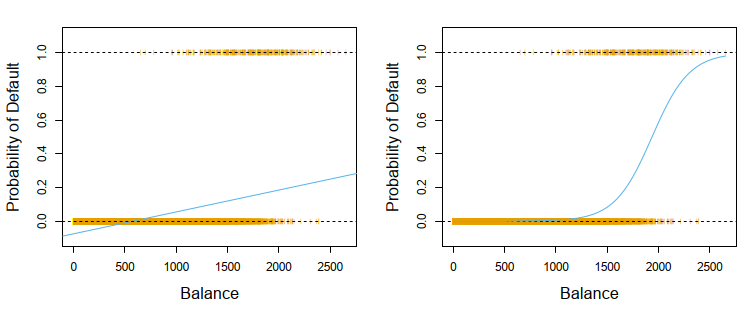
\includegraphics[width=0.8\textwidth]{figures/Linear_vs_logistic.png}
    \caption{Vergleich der geschätzten Wahrscheinlichkeiten für einen Testdatensatz zwischen linearer Regression (links) und logistischer Regression (rechts). \cite{James2023}}
    \label{fig:Vergleich_lin_log}
\end{figure}

Wie in \ref{fig:Vergleich_lin_log} zu sehen, können bei der linearen Regression die vorausgesagten Wahrscheinlichkeiten sogar negativ werden. Auch wird der gesamte Bereich von 0 bis 1 nicht ausgenutzt. Die logistische Regression löst dieses Problem. Um die benötigten Werte zwischen 0 und 1 vorherzusagen, setzt die logistische Regression die "logistische Funktion" ein:

\begin{equation}
    p(X) = \frac{e^{\beta_0 + \beta_1 X}}{1 + e^{\beta_0 + \beta_1 X}}
    \label{eq:logistische_funktion}
\end{equation}

Wie in Gleichung (\ref{eq:logistische_funktion}) zu sehen ist, nähert sich die Funktion für sehr große Werte von $X$ der 1 an und für sehr kleine Werte der 0. Durch Umformung lässt sich die logistische Funktion als lineares Modell formulieren. Der Ausdruck auf der linken Seite wird als Log-Odds bezeichnet:

\begin{equation}
    \log\left(\frac{p(X)}{1 - p(X)}\right) = \beta_0 + \beta_1 X
    \label{eq:log_odds}
\end{equation}

Wie in Gleichung (\ref{eq:log_odds}) ersichtlich ist, stellt das logistische Regressionsmodell sicher, dass der Logit linear von den Eingabevariablen $X$ abhängt.
Hierbei sind $\beta_0$ und $\beta_1$ die Koeffizienten oder Gewichte, die mit den Trainingsdaten bestimmt werden müssen. Das $X$ ist der Eingabewert (oder das Feature), dessen Zugehörigkeit bestimmt werden soll. Damit dies korrekt geschieht, wird die Maximum-Likelihood-Methode angewendet.

\begin{equation}
    l(\beta_0, \beta_1) = \prod_{i: y_i=1} p(x_i) \prod_{i': y_{i'}=0} (1 - p(x_{i'}))
    \label{eq:likelihood}
\end{equation}

Hierbei repräsentiert $p(x_i)$ die vorhergesagte Wahrscheinlichkeit für eine Beobachtung $i$, deren tatsächliche Klasse $y_i = 1$ ist, und $(1 - p(x_{i'}))$ die Wahrscheinlichkeit für eine Beobachtung $i'$, deren tatsächliche Klasse $y_{i'} = 0$ ist. Hat man die Koeffizienten erfolgreich bestimmt, muss man zum Klassifizieren nur noch den zu bestimmenden Wert in die X-Variable der logistischen Funktion einsetzen, um die Wahrscheinlichkeit zu erhalten, ob der Wert zu einer bestimmten Klasse gehört oder nicht.

Da in dieser Arbeit mit mehr als zwei Klassen gearbeitet wird, kommt die sogenannte multinomiale logistische Regression zum Einsatz. Es gibt hier verschiedene Ansätze, doch es läuft auf dasselbe Prinzip hinaus: Den einzelnen Klassen werden in ihrem Zusammenhang noch einmal einzelne Wahrscheinlichkeiten für ihren Eintritt zugewiesen. Dies geschieht entweder durch eine zufällig ausgewählte Klasse K als Basisklasse, mit der verglichen wird, oder komplett symmetrisch ohne eine einheitliche Referenz (die sogenannte Softmax-Methode).

Für die Methode mit $K$ Klassen und einer Klasse als Referenzklasse (hier Klasse $K$) berechnet man die Log-Odds für jede der verbleibenden $K-1$ Klassen im Verhältnis zu dieser Referenzklasse:

\begin{equation}
    \log\left(\frac{\Pr(Y=k|X=x)}{\Pr(Y=K|X=x)}\right) = \beta_{k0} + \beta_{k1}x_1 + \dots + \beta_{kp}x_p
    \label{eq:multinomial}
\end{equation}

Dabei beschreiben die Parameter $\beta_{k0}, \dots, \beta_{kp}$ die Koeffizienten spezifisch für die Klasse $k$.
Bei Softmax wird die Wahrscheinlichkeit für jede Klasse $k$ direkt berechnet, ohne eine Referenzklasse zu definieren:

\begin{equation}
    \Pr(Y=k|X=x) = \frac{e^{\beta_{k0} + \beta_{k1}x_1 + \dots + \beta_{kp}x_p}}{\sum_{l=1}^{K} e^{\beta_{l0} + \beta_{l1}x_1 + \dots + \beta_{lp}x_p}}
    \label{eq:softmax}
\end{equation}

Die Funktion in Gleichung (\ref{eq:softmax}) stellt sicher, dass die berechneten Wahrscheinlichkeiten für alle $K$ Klassen exakt auf 1 summieren. \footnote{\cite{James2023}}

Da es sich bei der logistischen Regression um eine vergleichsweise simple und transparente mathematische Funktion handelt, ist sie sehr leichtgewichtig. Sie arbeitet schnell, verbraucht nicht viel Speicher und lässt sich leicht in viele verschiedene Endgeräte integrieren. Daher wird sie in dieser Arbeit als erste Möglichkeit eingesetzt.

\subsection{Convolutional Neural Network}
Das Neural Network ist das Standardwerkzeug im Bereich des Deep Learning.

\begin{figure}[htbp]
    \centering
    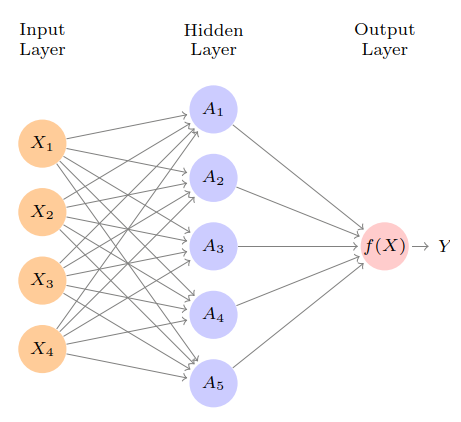
\includegraphics[width=0.6\textwidth]{figures/Neural_Network.png}
    \caption{Neural Network mit einem Hidden Layer. \cite{James2023}}
    \label{fig:neural_network}
\end{figure}

In seinen Grundsätzen besteht es aus einem Input Layer, einem oder mehreren Hidden Layern und einem Output Layer. Wie in Abbildung \ref{fig:neural_network} zu sehen ist, nimmt das Network eine Anzahl $p$ an Inputs $X = (X_1, \dots, X_p)$ und bildet im Hidden Layer eine nicht-lineare Transformation für die Kombination dieser Inputs in jedem Knoten $A$. Die Ergebnisse dieser sogenannten Aktivierungen werden an das Output Layer weitergereicht, um die nicht-lineare Funktion $f(x)$ zu bilden. Diese kann die Antwort $Y$ voraussagen. Die Aktivierungsfunktionen in den $K$ Knoten $A_k, k=1, \dots, K$ werden im Vorhinein festgelegt. Heutzutage verwendet man am häufigsten die ReLU-Funktion (Rectified Linear Unit):

\begin{equation}
    g(z) = (z)_+ = \begin{cases} 
        0 & \text{falls } z < 0 \\ 
        z & \text{sonst}
    \end{cases}
    \label{eq:relu}
\end{equation}

Diese ist einfacher zu berechnen und auch platzsparender als die vorher genutzte Sigmoid-Funktion. Das Modell aus Abbildung \ref{fig:neural_network} beschreibt, wie aus den fünf Kombinationen von $X$ fünf neue Features berechnet werden. Diese werden dann mit einer Aktivierungsfunktion transformiert. Am Ende ergibt sich ein lineares Modell zum Berechnen der Wahrscheinlichkeiten, ob ein Input zu einer Klasse gehört oder nicht.\footnote{\cite{James2023}}

Die meisten neuronalen Netze haben jedoch eine Vielzahl an Hidden Layern, um komplexere Aufgaben zu lösen, und auch mehrere mögliche Outputs, um Daten einer Vielzahl an möglichen Klassen zuzuordnen. Hierzu wird wieder die Softmax-Funktion aus Gleichung (\ref{eq:softmax}) verwendet, um für jede mögliche Klasse die Wahrscheinlichkeit zu errechnen, um dann den Input zur Klasse mit der höchsten Wahrscheinlichkeit zuzuweisen.

\begin{figure}[htbp]
    \centering
    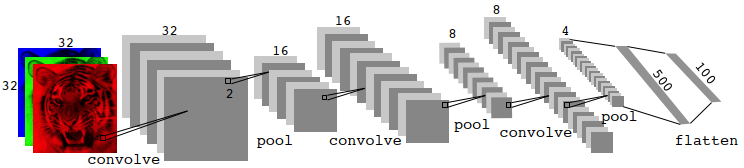
\includegraphics[width=0.8\textwidth]{figures/CNN.png}
    \caption{Struktur eines tiefen CNNs mit einer Abfolge von Convolutional Layers und Pooling Layers. \cite{James2023}}
    \label{fig:cnn}
\end{figure}

Das CNN zeichnet sich durch seine Eignung zur Klassifizierung mehrdimensionaler Daten aus. Anders als reguläre neuronale Netze werden die Hidden Layers hier in Convolutional Layers und Pooling Layers unterteilt. Diese Unterteilung ermöglicht ein hierarchisches Identifizieren von Features, von Low-Level nach High-Level, wobei mehrere Low-Level-Features zu High-Level-Features kombiniert werden, um schrittweise komplexere Muster zu erkennen. Die Convolutional Layers nutzen kleine Filtermatrizen (Kernels genannt), um schrittweise über die Daten zu gehen, die Werte, auf denen sie sich befinden, mit den Werten des Filters zu multiplizieren und die Produkte aufzusummieren. Je höher diese Summe, desto ähnlicher sind die originalen Daten dem Filter. Je niedriger, desto mehr unterscheiden sie sich. Während des Trainingsvorgangs passen sich die Filter an, um immer differenzierter lokale Muster zu erkennen und zu extrahieren. Als Ergebnis bekommt man eine Feature-Map, die die gefundenen Muster aufzeigt.

Das Pooling Layer fasst eine Feature-Map zu einem kleineren Bild zusammen. Mit dem Max-Pooling-Verfahren werden 2$\times$2-Blöcke an Daten erfasst und auf den höchsten vorhandenen Wert reduziert. So bleiben alle wichtigen Daten erhalten. Diese Schritte werden in mehreren aufeinanderfolgenden Layern wiederholt, bis die Feature Map auf ein Minimum reduziert wurde. Die Map wird dann von ihrer mehrdimensionalen Struktur in eine eindimensionale Reihe an Daten überführt und in ein neuronales Netz gespeist, ähnlich wie oben beschrieben. Am Ende erhält man wieder eine Reihe an Wahrscheinlichkeitsfunktionen für die möglichen Klassen.\footnote{\cite{James2023}}

Das CNN findet seine Anwendung meistens im Klassifizieren von Bildern und nicht in sequenziellen Datenreihen. Da beide aber in ihrer Struktur eine mehrdimensionale Abfolge an Daten darstellen, wird auch der Einsatz in diesem Fall untersucht.

\subsection{Long Short Term Memory}
Das LSTM gehört zur Gattung der Rekurrenten Neuronalen Netze (RNN) und ist darauf ausgelegt, einige fundementale Probleme die sowohl herkömmlichen CNNs als auch RNNs zu eigen sind zu lösen. Das RNN an sich setzt ein Konzept um, das den CNNs vorenthalten bleibt und theoretisch von hoher Bedeutung für diese Arbeit ist: das Behalten und Verwenden von vorher aufgenommenen Informationen zu einem späteren Zeitpung. Dies ermöglicht das Arbeiten mit sequentiellen Reihen an Daten, und das Verwenden früherer Zusammenhänge als Kontext für die Auswertung des Jetzigen, wie es sie in diesen Versuchen benötigt wird. Die Messreihe an Sensordaten stellt so eine Sequenz dar, und ist in ihrem Muster über einen Zeitraum aussagekräftiger als in den vereinzelten Ausschlägen ihrer Sensoren.

Doch das Problem mit herkömmlichen RNNs ist ihre Unfähigkeit Informationen über längere Zeitintervalle zu behalten. Josef Hochreiter hat dies in seiner 1997 erschienen Arbeit bereits thematisiert. In dieser spricht er vom sogenannten "decaying error back flow" (heute besser bekannt als das vanishing gradient problem), das bei zu langem Rückpropagieren der Fehler im Neuronalen Netz dazu führt, dass das Problem alsbald verschwindet und folglich die früheren Einheiten nichts mehr aus ihm lernen können. Analog hierzu ist das exploding gradient problem, bei dem der Fehler exponentiell ansteigt und so zu stark schwankenden Gewichten und unzuverlässigem Lernen führt. Um dieses Problem zu lösen, führt Hochreiter das "Constant Error Carousel" ein. Dieses wird in eine "Memory Cell" mit Input und Output Gates integriert. So können Informationen über lange Zeiträume gespeichert und für einen konstanten Fehlerfluss gesort werden. Die Gates sorgen dafür, dass nur relevante Informationen hinein und hinausgelangen. \cite{Hochreiter1997}

Moderne LSTMs lösen immer noch diese Probleme, haben jedoch einen abgewandelten Ansatz. In ihrer modernen Form (wie sie auch die in den Tests verwendete PyTorch Library implementiert) verfügen die Netze über sogenannte Forget Gates. Diese 1999 von Felix Gers beschriebenen Gates stellen sicher, dass die Memory Units des Netzes nicht fortwärend Daten ansammeln, die über die Zeit irrelevant werden. So werden Blöcke mit veralteten Daten resettet. \cite{Gers1999}

Ein weiterer Forstschritt sind die ebenfalls von Gers erfundenen "Peephole Connections", die dem Netz ermöglichen präzise Zeitabstände zu messen und Rhytmen vorherzusagen. \cite{Gers2000} Diese werden in dieser Arbeit, jedoch nicht verwendet.

\section{Verwandte Abhandlungen zur Klassifikation von Straßenqualität}
Im Review-Paper von Sattar et. al. werden verschiedene Studien ausgewertet und erfasst. Die Studien in diesem Paper handeln dabei hauptsächlich von Anomlie-Erfassungen wie Schlaglöcher, die die Fahrqualität und -sicherheit beeinflussen. Auch werden die Studien mit Autos und nicht mit Fahrrädern durchgeführt. \cite{Sattar2018} 

Dennoch lassen sich aus den aufgezählten Methoden und ihren Ergebnissen eine Methodik für die Versuche dieser Arbeit ableiten. Das Review geht auf die Komplikationen beim Sammeln der Daten ein: Smartphones verfügen über unterschiedliche Sensoren, Fahrzeuge haben unterschiedliche Gewichte und Abmaße die ihr Schwingungsverhalten beeinflussen. Auch die Geschwindigkeit, mit der ein Fahrzeug fährt, beeinflusst die aufgenommenen vertikalen Beschleunigungen - es kommt zu unterschiedlichen Vibrationsmustern in den Aufnahmen. Als Sensoren für die Aufnahmen verwenden die verschiedenen Autoren die Acceleratoren ihrer Geräte, während GPS und Gyroskop-Sensoren als komplementäre Daten. Rotation und Schwerkraft werden als mögliche Datenquellen genannt. Im Preprocessing werden zwei Ansätze zur Behandlung der unterschiedlichen Anbringungswinkel der Smartphones genannt: Das Transformieren des Geräte-Koordinatensystems auf ein lokales zum einen, und die Verwendung der gesamten Ausschlagsstärke aller drei Sensorachsen für ein im Raum unabhängiges Signal zum anderen. Um Störfaktoren in den Signalen zu entfernen und die Daten zu glätten werden verschiedene Filter verwendet, darunter high-pass butterworth, moving-average und band-pass. Zum Processing der Daten listen Sattar et. al. verschiedene Methoden der Forscher auf. Am häufigsten kommen Schwellenwertmethoden und ML zum Einsatz. Dem Problem mit der Geschwindigkeitsabhängigkeit der Signale wird ein Unterkapitel gewitmet. Einige Forscher normalisierten ihre Daten auf Referenzgeschwindigkeiten, andere teilten Geschwindigkeit in feste Kategorien ein, oder nutzen unterschiedliche Algorithmen je nach Geschwindigkeit. Keines dieser Methoden führte zu einer kompletten Lösung des Problems, sodass der Einfluss der Geschwindigkeit vollständig ausgeglichen wäre. \cite{Sattar2018}

Die Autoren des Reviews kommen zu dem Ergebnis, dass die Erkennungsmethoden nur in weitem Maße anwendbar sind, wenn ihre Daten aus einer Vielzahl von Zuständen stammen. Verschiedene Fahrzeuge (in diesem Fall Autos), verschiedene Smartphone-Modelle und Geschwindigkeiten werden empfohlen. Ebenso wird auf die Wichtigkeit einer korrekten Vorverarbeitung der Daten hervorgehoben. Die meisten Forscher verwenden starre Setups für ihre Smartphones. Die Autoren fordern eine variable Aufhängung der Geräte zu ermöglichen und die Differenzen per Transformation auszugleichen. \cite{Sattar2018}

Im Review stellte sich die Herangehensweise mit ML als verlässlicher heraus als die Schwell-wert-Methoden. Es wird darauf hin-gewiesen, dass viele Autoren nur einen einzelnen Sensor ihres Smartphones für die Aufnahmen genutzt haben. Sattar et al. empfehlen eine Herangehensweise über Datenfusion von verschiedenen Sensoren, darunter Linear Acceleration (die Accelerometer-daten, aus denen die Schwerkraft bereits herausgerechnet wurde), Gyroskop und Schwerkraftsensor. Um das Problem mit den Diskrepanzen zwischen verschiedenen Test-Setups zu dämpfen wird Anwendung von Crowdsourcing empfohlen. Anwender konnten eine signifikante Steigerung ihrer Accuracy verzeichnen. In diesem Zusammenhang wird aber auch von den Ungenauigkeiten gewarnt, die von Positionsdaten herrüren, die von Mobilnetz und GPS bezogen werden. \cite{Sattar2018}

In ihrem Bericht gehen Seraj et al. näher auf ihre eigene Problematik mit Geschwindigkeitsverarbeitung ein. Sie verwenden ebenfalls Autos für ihre Aufnahmen und fokusieren sich auf Straßenanomalien, doch die Problematik bleibt auch für diese Arbeit relevant. Es wird darauf eingegangen, dass das GPS des Smartphones zur Verarbeitung der Geschwindigkeit verwendet wurde. Es stellte sich heraus, dass die erforderlichen Signale nicht immer erhältlich waren. Auch leiden GPS unter der sogenannten TTFF (time to first fix), die benötigt wird, um die Position über das Satellitensignal zu bestimmen. Im Falle komplett fehlender GPS Daten griffen die Autoren auf eine andere Tachnik zurück: die Hüllkurvendemodulation. Sie stellen fest, dass Komponenten wie Geschwindigkeit, Drift und Steigung im Signal der Accelerometer enthalten ist und können sie mit der Demodulation herausfiltern. \cite{Seraj2016}

Heidt und Dorer klassifizieren Fahrradstrecken nach drei verschiedenen Bodenbelägen - Asphalt, Pflasterstein und Kies zu je drei Qualitätsabstufungen. Hierfür benutzen sie ein industrielles Sensorgerät der Firma Bosch, das sie in Fest mit dem Rahmen des Fahrrads verbauen, um sekundäre Bewegungen zu unterbinden. Als Quellen für ihre Features verwenden sie Acceleratoren und Gyroskop des Geräts. Für ihre Deep Learning Modelle verwendeen sie die rohen x-, y- und z-Werte der Daten, die lediglich genormt werden. Für die anderen Methoden werden aus den Rohdaten Arithmetisches Mittel, Standardabweichung, Maximal- und Minimalwert, mittlere Breite und Amplitude der Signalspitzen, mittlerer Spitzenabstand, mittlere positive und negative Steigung sowie maximale positive und minimale negative Steigung abgeleitet. Sie nehmen mit einer Sensorrate von bis zu 300 Hz auf und testen ihren Messreihen mehrere verschiedene Klassifikatoren. Zu ihnen gehören XGBoost, Random Forest, Support Vector Machine (SVM), CNN, LSTM, ein CNN-LSTM Modell, ein ResNet Modell und ein InceptionTime Modell. Für alle Modelle versuchen sie eine Vielzahl an Kombinationen der Hyperparameter, um die beste Accuracy beim Klassifizieren ihrer Testdaten zu erzielen. Mit optimierten Einstellungen erreichen die Residual Net Modelle eine Accuracy von 99\%. Vor allem höhere Aufnahmefrequenzen um ca. 300Hz erweisen sich als besser. Bei den niedrigeren Frequenzen sind Signale rauer Oberflächen verschiedener Bodenklassen schwerer zu unterscheiden. Die auf diese Weise trainierten Modelle stellen sich jedoch als nicht transferierbar heraus. Beim Testem mit einem anderen Fahrrad erreichen die besten Modelle eine Accuracy von nur 26\%. \cite{Heidt2021} Das von Heidt und Dorer beschriebene Vorgehen und die verwendeten Modelle dienen dieser Arbeit als Inspiration. Auch soll mit dem Verwenden einer handelsüblichen Handyhalterung mit einer loseren Verbindung zum Fahrrad ein transferierbareres Modell geschaffen werden. Das Paper von Heidt und Dorer weisen jedoch auf die große Herausforderung hin, die diese Transferierbarkeit darstellt. (Diskussion für Transferierbarkeit, Einstellungen für verschiedene Fahrräder, Aufnahmefrquenz)

In der Abhandlung von Massow et. al. wird komplett auf Machine Learning verzichtet. Das Ziel der Autoren ist es, eine allgemein nutzbare Methode zum Erfassen von Straßenqualität über Handysensoren während des Fahrradfahrens zu finden. Hierfür vergleichen sie verschiedene Berechnungsmethoden und führen in detaillierten Schritten die Vorverarbeitung der Daten vor. Als Berechnungsmethoden werden verglichen: den Pavement Condition Index (PCI), der über das Zählen von Anomalien in der Straße erhalten wird, der International Roughness Index (IRI) in verschiedenen Varianten, basierend auf dem quadratischen Mittelwert der Sensorbeschleunigungen, und die über die Fourier Transformation gewonnene Power Spectral Density (PSD) für Frequenzanalysen. Verglichen wird die Fähigkeit der verschiedenen Methoden, eine Teststrecke mit drei distinktiven Abschnitten - erst Pflastersteine, dann Asphalt, dann Gehweg - sichtbar in ihrer Qualität zu unterscheiden. In der Auswertung geht der IRI in einer Variante, in der er mit der durchschnittlichen Geschwindigkeit über eine festgelegte Distanz verrechnet wird als Sieger hervor, da er Straßen in Abstufung von Schlecht, Mittelgut und Gut verlässlich und in Abstufungen unterscheiden kann. Die genaue Art des Belags wird dabei nicht unterschieden. \cite{Massow2024} Diese Arbeit baut auf den Ergebnissen und Herangehensweisen Massows und seines Teams auf.

Tarkiainen und Ikonen haben eine Studie zu Einflussfaktoren auf die Aufnahme von Smartphonesenoren beim Fahrradfahren durchgeführt. Wie auch in dieser Arbeit wird das Smarphone mit einer Halterung am Lenker montiert, um verschiedene Faktoren wie den Neigungswinkel, die Aufnahmefrequenz und den Fahrradtyp zu testen. Dabei werden die Daten nicht klassifiziert, sondern statistisch und visuell in Matlab analysiert. Sie kommen zu dem Ergebnis, dass eine horizontale Aussrichtung des Smartphones auf dem Lenker, parallel zur Erdoberfläche, die besten Ergebnisse für Acceleratoren-Messungen hervorbringt. Das abgewinkelte Smartphone führt zu sichtbar gedämpften Ausschlägen der Acceleratoren im Vergleich zum horizontal montierten Smartphone. Ähnliche Effekte sind bei den Mittelwerten und der Standardabweichung der Acceleratoren zu sehen. Auch kommt das Paper zu dem Entschluss, dass eine niedrigere Aufnahmefrequenz weniger "Noise" in die Daten bringt. Dies bietet Vorteil für die visuelle Erfassung, womit begründet wird, dass eine höhere Aufnahmefrequenz nicht unbedingt besser ist. Von Interesse ist auch die Berechnung der Acceleratorenfrequenz im vertikalen Bereich, die anders als bei Massow über eine Projektion des Accelerationsvektors in Richtung des Schwerkraftvektors erfolgt. \cite{Tarkiainen2025}

Da das Paper sich mit der Analyse von Anamolien auf der Straße im Allgemeinen befasst und nicht um die Bestimmung verschiedener Beläge wird in dieser Arbeit eine höhere Aufnahmefrequenz gewählt, um feinere Unterschiede feststellen zu können. Auch wird das Smartphone in einem Winkel positioniert, was zwar für die Messungen suboptimal ist, aber eine deutlich natürlichere Position für den alltäglichen Gebrauch darstellt.

